\section{Reinforcement learning}

Reinforcement learning is an approach to the learning from experience problem in artificial intelligence. A reinforcement learning algorithm uses past experiences and domain knowledge to make intelligent decisions in the future \parencite{barto1998reinforcement}.

\begin{figure}[htbp]
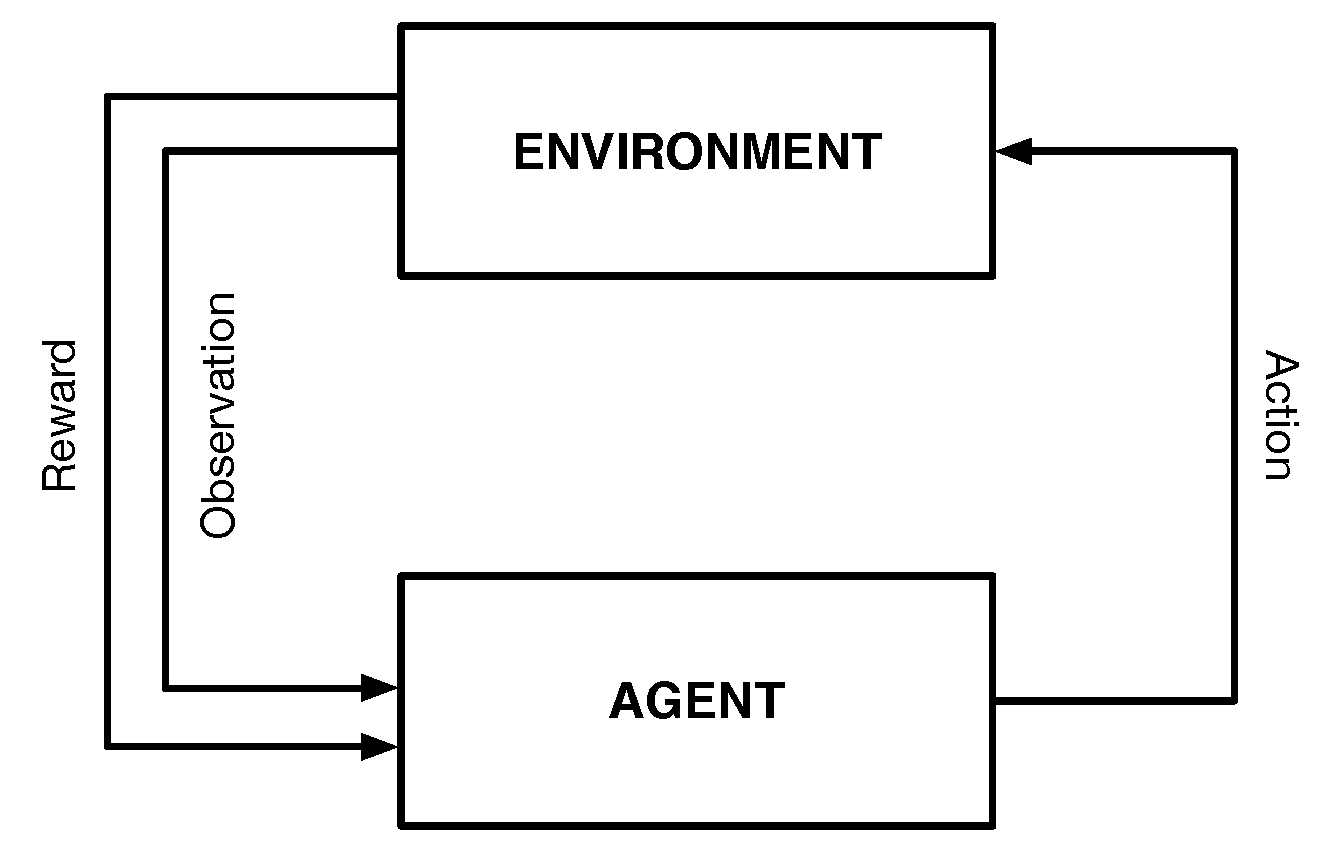
\includegraphics[width=\textwidth]{images/agent-environment.pdf}
\caption{The reinforcement learning process}
\label{fig:agentandenvironment}
\end{figure}

The reinforcement learning problem is modeled as a sequential decision problem, see figure \ref{fig:agentandenvironment} for a graphical representation of the process. A learning agent performs an action and receives a reward according to some measure of how desirable the results of the action are.  After the action is taken, the state of the environment changes and the agent then receives a new observation and the process repeats. The goal of the reinforcement learning agent is to maximize the reward received over a certain time period, the horizon time, finding a balance between immediate and future rewards \parencite{barto1998reinforcement}. 

There are several ways of further dividing reinforcement learning problems into other subcategories. Some examples are the dichotomies episodic/non-episodic problems, problems with continuous/discrete state spaces, problems with continuous/discrete action spaces, problems with one/multiple concurrent agents etc. In the text below, the two first of these dichotomies, which are relevant to this thesis, are discussed. 

\subsection{Episodic and non-episodic problems}
One can categorize reinforcement learning problems based on whether or not the time steps are divided into episodes. If they are, the problem is called episodic, and otherwise it is called non-episodic. Episodic problems are common in for example games, which end when they are won or lost. An episode here corresponds to a full game from start to finish. In a non-episodic problem, the interaction between the actor and environment goes on continuously without end \parencite{barto1998reinforcement}. Two examples of non-episodic applications are controlling a robot arm (as well as other robotics problems) and maneuvering a helicopter \parencite{ng2006autonomous}. 

\subsection{Continuous and discrete problems}
An alternative way to categorize reinforcement learning problems is based on whether their state spaces are continuous or discrete. An important difference between the two kinds of problems is how an agent can treat similar states in the model. In a continuous problem it is a lot easier to group together states located around the same ``position'' due to the nature of a continuous problem, where the states usually more or less meld together. For example, if the reinforcement learning problem is to control a robot arm whose position constitutes the state of the environment, the states located around the same general area are not very different. This means that they might be treated in the same way or a similar way by an agent. On the other hand, consider the discrete problem of a game of chess, wherein the placement of a pawn in one of two adjacent squares could dramatically change the evaluation of the state and the outcome of the game \parencite{barto1998reinforcement}.
